\documentclass[english,man]{apa6}

\usepackage{amssymb,amsmath}
\usepackage{ifxetex,ifluatex}
\usepackage{fixltx2e} % provides \textsubscript
\ifnum 0\ifxetex 1\fi\ifluatex 1\fi=0 % if pdftex
  \usepackage[T1]{fontenc}
  \usepackage[utf8]{inputenc}
\else % if luatex or xelatex
  \ifxetex
    \usepackage{mathspec}
    \usepackage{xltxtra,xunicode}
  \else
    \usepackage{fontspec}
  \fi
  \defaultfontfeatures{Mapping=tex-text,Scale=MatchLowercase}
  \newcommand{\euro}{€}
\fi
% use upquote if available, for straight quotes in verbatim environments
\IfFileExists{upquote.sty}{\usepackage{upquote}}{}
% use microtype if available
\IfFileExists{microtype.sty}{\usepackage{microtype}}{}

% Table formatting
\usepackage{longtable, booktabs}
\usepackage{lscape}
% \usepackage[counterclockwise]{rotating}   % Landscape page setup for large tables
\usepackage{multirow}		% Table styling
\usepackage{tabularx}		% Control Column width
\usepackage[flushleft]{threeparttable}	% Allows for three part tables with a specified notes section
\usepackage{threeparttablex}            % Lets threeparttable work with longtable

% Create new environments so endfloat can handle them
% \newenvironment{ltable}
%   {\begin{landscape}\begin{center}\begin{threeparttable}}
%   {\end{threeparttable}\end{center}\end{landscape}}

\newenvironment{lltable}
  {\begin{landscape}\begin{center}\begin{ThreePartTable}}
  {\end{ThreePartTable}\end{center}\end{landscape}}

  \usepackage{ifthen} % Only add declarations when endfloat package is loaded
  \ifthenelse{\equal{\string man}{\string man}}{%
   \DeclareDelayedFloatFlavor{ThreePartTable}{table} % Make endfloat play with longtable
   % \DeclareDelayedFloatFlavor{ltable}{table} % Make endfloat play with lscape
   \DeclareDelayedFloatFlavor{lltable}{table} % Make endfloat play with lscape & longtable
  }{}%



% The following enables adjusting longtable caption width to table width
% Solution found at http://golatex.de/longtable-mit-caption-so-breit-wie-die-tabelle-t15767.html
\makeatletter
\newcommand\LastLTentrywidth{1em}
\newlength\longtablewidth
\setlength{\longtablewidth}{1in}
\newcommand\getlongtablewidth{%
 \begingroup
  \ifcsname LT@\roman{LT@tables}\endcsname
  \global\longtablewidth=0pt
  \renewcommand\LT@entry[2]{\global\advance\longtablewidth by ##2\relax\gdef\LastLTentrywidth{##2}}%
  \@nameuse{LT@\roman{LT@tables}}%
  \fi
\endgroup}


  \usepackage{graphicx}
  \makeatletter
  \def\maxwidth{\ifdim\Gin@nat@width>\linewidth\linewidth\else\Gin@nat@width\fi}
  \def\maxheight{\ifdim\Gin@nat@height>\textheight\textheight\else\Gin@nat@height\fi}
  \makeatother
  % Scale images if necessary, so that they will not overflow the page
  % margins by default, and it is still possible to overwrite the defaults
  % using explicit options in \includegraphics[width, height, ...]{}
  \setkeys{Gin}{width=\maxwidth,height=\maxheight,keepaspectratio}
\ifxetex
  \usepackage[setpagesize=false, % page size defined by xetex
              unicode=false, % unicode breaks when used with xetex
              xetex]{hyperref}
\else
  \usepackage[unicode=true]{hyperref}
\fi
\hypersetup{breaklinks=true,
            pdfauthor={},
            pdftitle={Acoustic Correlates of Stress in Lithuanian},
            colorlinks=true,
            citecolor=blue,
            urlcolor=blue,
            linkcolor=black,
            pdfborder={0 0 0}}
\urlstyle{same}  % don't use monospace font for urls

\setlength{\parindent}{0pt}
%\setlength{\parskip}{0pt plus 0pt minus 0pt}

\setlength{\emergencystretch}{3em}  % prevent overfull lines

\ifxetex
  \usepackage{polyglossia}
  \setmainlanguage{}
\else
  \usepackage[english]{babel}
\fi

% Manuscript styling
\captionsetup{font=singlespacing,justification=justified}
\usepackage{csquotes}
\usepackage{upgreek}

 % Line numbering
  \usepackage{lineno}
  \linenumbers


\usepackage{tikz} % Variable definition to generate author note

% fix for \tightlist problem in pandoc 1.14
\providecommand{\tightlist}{%
  \setlength{\itemsep}{0pt}\setlength{\parskip}{0pt}}

% Essential manuscript parts
  \title{Acoustic Correlates of Stress in Lithuanian}

  \shorttitle{Lithuanian Stress}


  \author{Christopher Oakden\textsuperscript{1}}

  % \def\affdep{{""}}%
  % \def\affcity{{""}}%

  \affiliation{
    \vspace{0.5cm}
          \textsuperscript{1} Rutgers University  }

  \authornote{
    Correspondence concerning this article should be addressed to
    Christopher Oakden, 18 Seminary Pl. New Brunswick, NJ 08901. E-mail:
    \href{mailto:chris.oakden@rutgers.edu}{\nolinkurl{chris.oakden@rutgers.edu}}
  }


  \abstract{This paper presents the results of a production experiment examining the
acoustic correlates of word stress in Lithuanian, a language which also
exhibits lexical tone contrasts. Analysis of the data indicates that
duration and intensity are reliably perceptible markers of stress
(consistent with previous impressionistic descriptions), but vowel
quality (as measured by F1 and F2) is not. Pitch (F0) data collected in
the study are ambiguous between stress correlate and categorical tonal
target, and are therefore inconclusive. Data from more speakers is
therefore necessary to disambiguate the two possibilities.}
  \keywords{Stress Correlates, Stress and Tone, Lithuanian \\

    \indent Word count: 3970
  }




  \usepackage{tipa}
  \usepackage{gb4e}
  \noautomath

\usepackage{amsthm}
\newtheorem{theorem}{Theorem}
\newtheorem{lemma}{Lemma}
\theoremstyle{definition}
\newtheorem{definition}{Definition}
\newtheorem{corollary}{Corollary}
\newtheorem{proposition}{Proposition}
\theoremstyle{definition}
\newtheorem{example}{Example}
\theoremstyle{definition}
\newtheorem{exercise}{Exercise}
\theoremstyle{remark}
\newtheorem*{remark}{Remark}
\newtheorem*{solution}{Solution}
\begin{document}

\maketitle

\setcounter{secnumdepth}{0}



\section{Background}\label{background}

The purpose of the current study is to answer the question:
\enquote{What is stress in a tone/pitch accent language?} Convergence of
metrical structure and lexical tone on a single language poses a
relevant question for phonetic implementation: given that perturbation
in fundamental frequency (F0) is a correlate of tone \textit{and} of
stress (see Gordon and Roettger (2017) for a cross-linguistic survey of
stress correlates), which acoustic properties will stress utilize in a
language which also contrasts for tone?

To address this question, a production study was performed to examine
the acoustic correlates of stress in Lithuanian, a language which is
reported to exhibit both word stress and lexical pitch accent(tone), as
well as an interaction between tone and stress (see Blevins (1993),
deLacy (2002) and numerous references cited therein). Impressionistic
descriptions of stress in the language include increases in duration,
loudness, and pitch, as well as qualitative changes in vowels, with
tonal contrasts being neutralized in unstressed position (see Ambrazas
(1997), Girdenis (2003), and Young (1991)).

Disagreement exists in the literature regarding the tonal inventory of
the language. Generative accounts posit a three-way tonal distinction:
falling (\textit{acute}) and rising (\textit{circumflex}) pitch accents
realized on syllables with long vowels, diphthongs or sonorant codas,
and a shorter falling (\textit{grave}) pitch accent on syllables with
short vowels or obstruent codas (Kenstowicz (1972), deLacy (2002)).
Structuralist descriptions of the language (Mathiassen (1996), Ambrazas
(1997), Girdenis (2003)) maintain that since grave syllables are not
contrastive, they do not constitute proper pitch accents, and are merely
the realization of word stress. To establish an acoustic profile of
stress, and in an attempt to maximally disambiguate stress from tone,
the experiment limited its focus to grave syllables.

\section{Methods}\label{methods}

This section outlines the details of the production experiment from
which acoustic data were gathered, describes data processing procedures,
and identifies the framework for statistical analysis.

\subsection{Participants}\label{participants}

Data from four native speakers of Lithuanian was collected, of which one
was used for analysis in the current study. Information about the
speaker was gathered via a demographic questionnaire instrument which
the participant completed before beginning the experiment. This speaker
(male, mid 30s) was born in Lithuania and acquired the language as his
L1 during childhood, moving to the United States after reaching
adulthood. His primary home language continues to be Lithuanian, which
he speaks daily with his spouse (also an L1 Lithuanian speaker) and
children (heritage speakers). This suggests a low possibility of L1
attrition. Additionally, the subject was naïve to the purpose of the
study, was not trained in linguistics, and had no history of speech
impairment.

\subsection{Target Stimuli}\label{target-stimuli}

Multiple segmental and prosodic controls were implemented during
selection of target stimuli (n = 60), which were limited to nominal
forms (roots+inflectional suffixes). The primary control limited targets
to a specific syllabic structure and default stress placement:
trisyllabic words of the shape {[}CVCVCV(C){]} and tetrasyllabic words
of the shape {[}CVCVCVCV(C){]}, with default stress on the penult.
Potential targets with complex onsets in any position (pre-tonic, tonic,
post-tonic) were excluded. Additionally, target selection minimized root
syllables containing codas {[}CVC{]} or lacking onsets {[}V{]}. Due to
lexical gaps, however, two target roots were selected which contained
these suboptimal structures: \textit{apetit}- \enquote{apetite} and
\textit{mygtuk}- \enquote{button}.

Syllables containing the short vowels {[}u{]} and {[}i{]} were given
preference in selection (n = 32 and 28, respectively), as these vowels
are not reported to undergo phonological lengthening in stressed
position, an effect reported for the vowels {[}a{]} and {[}e{]}
(Kenstowicz (1972), Ambrazas (1997), Girdenis (2003)).

Segmental environment on the vowel in the stressed syllable was also
controlled. Grave syllable vowels were flanked by either stops {[}k, t,
p{]}--and to a lesser extent {[}g{]} and {[}d{]}--(n = 36) or sonorants
{[}l, m, n{]} (n = 24). Again, the prevalence of lexical gaps prevented
controlling for either stop or sonorant segments exclusively, so
segmental environment was coded as a variable in statistical analysis.

Targets conforming to the above restrictions were further limited to
roots of the same declension class (Ia) and accent class (2) to ensure
uniformity of accentual properties across stimuli (see Ambrazas (1997)
for more discussion). Four suffixes from this declension class were
selected to combine with nominal roots based on predicted stress
placement: two suffixes (nominative singular {[}-as{]} and genitive
singular {[}-o{]}) for which stress is predicted to surface on the
default root position, and two suffixes (locative singular {[}-e{]} and
accusative plural {[}-us{]}) for which stress is predicted to surface on
the suffix (also known as a \emph{stress mobility} effect; see Blevins
(1993), Dogil (1999), Ambrazas (1997), Girdenis (2003), Mathiassen
(1996), and Young (1991) for more discussion).

\subsection{Scenario/Frame Sentences}\label{scenarioframe-sentences}

Target words were placed within two frame sentences designed to illicit
vernacular speech production. Participants were asked to imagine
themselves in an informal conversation with a friend in a restaurant or
bar setting. The subject notices that someone has scrawled a word on the
wall next to them, making an observation about the strange appearance of
the handwriting. Subjects read each target word in both frame sentences,
provided in (1).

\newpage

\begin{exe}
\ex
\begin{xlist}
\ex\label{ex1a}
\glll \v{Z}iurek, \v{c}ia para\v{s}ytas \v{z}odis [target]. \\
\textipa{ZuRek} \textipa{\t{tS}a} \textipa{p\super haRaSi:tas} \textipa{Zodis} {} \\
look there write.\textsc{pass} word {} \\
\glt `Look, the word [target] is written over there.'
\vspace{.5cm}
\ex\label{ex1b}
\glll \v{Z}odis [target] para\v{s}ytas keistai. \\
\textipa{Zodis} {} \textipa{p\super haRaSi:tas} \textipa{k\super heistai} \\
word {} write.\textsc{pass} strange \\
\glt `The word [target] is written strangely.'
\end{xlist}
\end{exe}

Designing a scenario which focuses on a written word in the ambient
environment allowed the frame sentences to accommodate any word equally
well, regardless of its declension. The target word appears
sentence-finally in the first frame sentence and sentence-medially in
the second frame. To control for any confounds related to phrase-final
lengthening (Wightman, Shattuck-Hufnagel, Ostendorf, and Price (1992)),
frame sentence was coded as a variable in the statiscial models.

\subsection{Procedure}\label{procedure}

Recording took place inside a sound-attenuated booth at the Phonology
and Field Research Laboratory at Rutgers University. The subject wore an
AKG C420 head-worn microphone with behind-the-neck headband to maintain
constant distance from the mouth. Sound recordings were made with
GoldWave v6.10 software at 44.1k Hz sampling rate and 16-bit quantizing
resolution in mono. Experiment prompt images were projected onto a
laptop screen inside the recording booth. The images portrayed a scene
with non-descript characters dining in a restaurant/bar setting, one of
which is shown pointing to a word in strange handwriting in the ambient
environment. The same word appeared at the top left-hand corner of the
screen in standard orthography, as shown in \textit{Figure 1}.

\begin{figure}
\centering
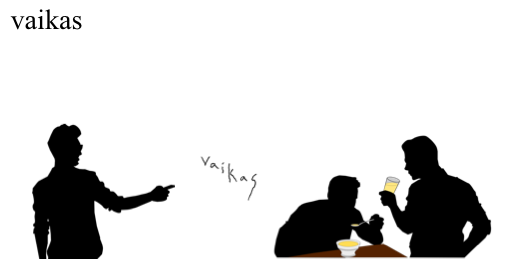
\includegraphics{../figs/Picture1.png}
\caption{Example prompt}
\end{figure}

Frame sentences were printed on a separate sheet of paper for the
participant's reference. The subject read the word in both frame
sentences, then pressed a key to advance to the next picture. Three
repetitions of the stimuli (situated within both frame sentences) were
recorded. Target order was randomized and counterbalanced in each
repetition, with filler words evenly spaced among stimuli. Five
additional fillers were placed at the beginning of each repetition to
accommodate any initial hyper- or mis-articulation in case the
participant felt anxious about the task. All three repetitions were
completed during a single session with a 10-to-15 minute break between
each repetition.

\subsection{Exclusions}\label{exclusions}

60 target words were produced within 2 frame sentences across 3
repetitions, totaling 360 individual productions of stimuli. Of these,
12 productions (6 target productions across 2 frame sentences) were
excluded from analysis due to stuttering or excessive pausing. These
include 4 target productions from the first repetition, 2 from the
second repetition, and 6 from the third repetition.

\subsection{Hypotheses}\label{hypotheses}

The current study tests the following hypotheses (2), which are based on
traditional descriptions of the acoustic realization of word stress in
Lithuanian.

\begin{exe}
\ex \textit{Experiment Hypotheses}\
\begin{xlist}
\ex\label{ex1a} Hypothesis 1: Duration of vowels in stressed syllables is \textbf{longer} than in unstressed syllables \
\ex\label{ex1b} Hypothesis 2: Intensity of vowels in stressed syllables is \textbf{greater} than in unstressed syllables \
\ex\label{ex1c} Hypothesis 3: Vowels in stressed syllables are \textbf{more peripheralized} (as measured by F1 and F2) than in unstressed syllables \
\ex\label{1d} Hypothesis 4: Pitch (as measured by F0) in stressed syllables is \textbf{higher} than in unstressed syllables
\end{xlist}
\end{exe}

\subsection{Data Processing}\label{data-processing}

After data collection concluded, sound files were annotated using
TextGrids in Praat (Boersma and Weenink (2016)). Boundaries were marked
for all vowels within target words as well as fixed intervals in both
frame sentences for the purpose of duration normalization. Left edges
were identified by placing a boundary at the zero crossing of the first
periodic, non-deformed waveform of the vowel (Francis, Ciocca, and Yu
(2002)). The right edges of vowels were determined by inserting a
boundary at the end of the vowel's second formant (Turk, Nakai, and
Sugahara (2006)).

TextGrid intervals were marked to indicate a) the vowel, b) predicted
stress pattern based on traditional accounts, c) position within the
word or frame sentence, and d) number of syllables of the target word.
File names were coded to indicate the repetition (A = 1st repetition, B
= 2nd repetition, C = 3rd repetition). These factors formed the basis
for the fixed and random effects structure of the statistical analysis.

Duration data were extracted using boundary marks on TextGrids for each
audio file. A normalization multiplier was created by dividing the raw
duration of the marked fixed interval in each frame sentence by the mean
of all fixed intervals. This yielded 128 target repetition- and frame
sentence-specific multipliers. TextGrid intervals for vowels in each
target word in a given frame sentence were multiplied by the
corresponding multiplier, yielding a normalized value. Intensity, F1,
F2, and F0 data were collected using a modified Praat script based on
Lennes (2003). Vowel midpoint values were extracted for each acoustic
parameter to ensure measurement of the most stable portion of the vowel.
Two datapoints for the vowel {[}u{]} failed to return F0 measurements,
and were discarded.

A subset of the data were isolated for analysis. This includes {[}u{]}
and {[}i{]} vowels in penultimate position on nominals. Traditional
descriptions predict stress to fall on the root when combining with
nominative singular and genitive singular suffixes, and on the suffix
when combining with locative singular and accusative plural suffixes.
This allows for direct comparison of the acoustic properties of vowels
which are predicted to be in both stressed and unstressed positions. An
example is given in (3) of the root \emph{ratuk-} \enquote{wheel}, with
the syllable containing the relevant vowel in bold.

\begin{exe}
\ex \textit{Predicted Stress} \
\begin{xlist}
\ex\label{ex1a} ra.\textipa{"}\textbf{tu}.kas `wheel \textsc{NomSg}' (stress predicted on root) \
\ex\label{ex1b} ra.\textbf{tu}.\textipa{"}kus `wheel \textsc{AccPl}' (stress predicted on suffix)
\end{xlist}
\end{exe}

\subsection{Statistical Analysis}\label{statistical-analysis}

A series of linear mixed effects models were fit to the data using the
\emph{lmer()} function in the lme4 package (Bates, Mächler, Bolker, and
Walker (2015)) in R (R Core Team (2017)). For each vowel, five separate
models were fit. Acoustic parameter (normalized duration, intensity, F1,
F2, and F0) was set as the criterion, with four categorial variables set
as predictors: predicted stress (stressed and unstressed), frame
sentence (1st frame sentence and 2nd frame sentence), segmental
environment of the vowel (obstruents and sonorants), and syllable count
of the word (three syllables and four syllables). The random effects
structure for each model specified by-word random slopes for segmental
environment, frame sentence, and repetition.

To test for the effect of predicted stress (as described in traditional
accounts) on the acoustic realization of each parameter, nested models
were created for each of the five models which excluded the predicted
stress predictor. Corresponding models were then compared via a
Likelihood Ratio Test using R's \emph{anova()} function, yielding a
p-value. Experiment-wise alpha was set at 0.05.

All models converged with full specification, and visual inspection of
residual plots for the normalized duration, intensity, F1, and F2 models
did not indicate any violation of homoskedasticity or normality. The F0
models did, however, violate this assumption. This will be explored in
further detail in the Discussion section.

\section{Results}\label{results}

This section presents the results of the experiment. Results of each
acoustic correlate (normalized duration, intensity, F1/F2, F0) are
presented separately.

\subsection{Normalized Duration}\label{normalized-duration}

Mean values of normalized duration and standard deviation show variation
as a function of predicted stress. Stressed syllables were longer in
duration than unstressed syllables, and this generalization was true for
both {[}u{]} and {[}i{]}, as shown in \textit{Figure 2}.

\begin{figure}
\centering
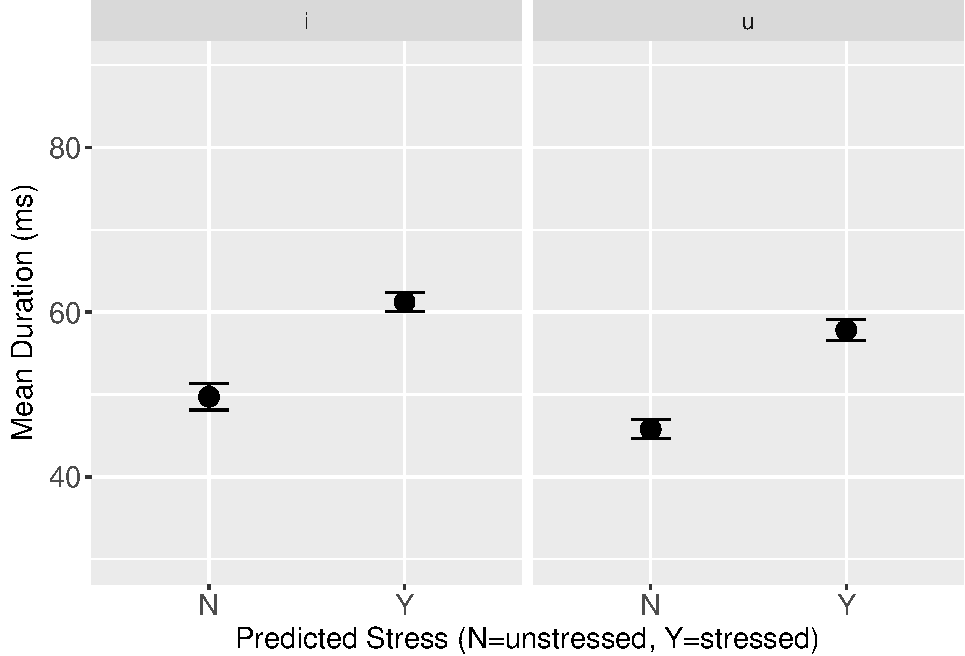
\includegraphics{lithuanian_article_files/figure-latex/Figure2-1.pdf}
\caption{\label{fig:Figure2}Mean Normalized Duration in ms by Predicted
Stress (N=unstressed, Y=stressed), {[}u{]} and {[}i{]}}
\end{figure}

Specifically, {[}u{]} vowels in stressed position exhibited a mean
normalized duration of 57.5 ms (13.0 ms s.d.), with unstressed vowels
approximately 12ms shorter (mean normalized duration of 45.6 ms and 10.8
ms s.d.). This effect was observed across frame sentences and for both
three- and four-syllable words (see \textit{Table 1}). Model comparison
with linear mixed effects models fit to the data confirmed the effect of
predicted stress on the normalized duration of {[}u{]}
(\(\chi^2(1) = 33.163, p < 0.05\)). Predicted stress on {[}u{]} vowels
corresponds with an estimated duration increase of 11.62 ms +/- 3.51 ms
(standard error).

\begin{table}

\caption{\label{tab:Table1}Normalized Duration in ms by Predicted Stress (Stress), Frame Sentence (Frame), and Syllable Count (Syllnum), [u] Vowel}
\centering
\begin{tabular}[t]{l|r|l|r|r}
\hline
Stress & Frame & Syllnum & Mean & SD\\
\hline
N & 1 & four & 47.06 & 13.00\\
\hline
N & 1 & three & 46.03 & 12.54\\
\hline
N & 2 & four & 44.52 & 9.07\\
\hline
N & 2 & three & 44.97 & 8.96\\
\hline
Y & 1 & four & 61.51 & 12.68\\
\hline
Y & 1 & three & 58.07 & 12.87\\
\hline
Y & 2 & four & 52.87 & 12.43\\
\hline
Y & 2 & three & 57.29 & 13.51\\
\hline
\end{tabular}
\end{table}

Difference in mean normalized duration for {[}i{]} vowels between
stressed (62.8 ms, 13.5 ms s.d.) and unstressed (47.9 ms, 12.7 ms s.d.)
syllables collapsed across other categories was approximately 14.9 ms.
Mean values grouped by frame sentence and by-word syllable count are
shown in \textit{Table 2}. Predicted stress was determined to be a
significant effect for these values as a result of model comparison
(\(\chi^2(1) = 28.298, p < 0.05\)). Stress on syllables with a {[}i{]}
nucleus correlated with a 12.85 ms increase in normalized duration +/-
2.26 ms (standard error).

\begin{table}

\caption{\label{tab:Table2}Normalized Duration in ms by Predicted Stress (Stress), Frame Sentence (Frame), and Syllable Count (Syllnum), [i] Vowel}
\centering
\begin{tabular}[t]{l|r|l|r|r}
\hline
Stress & Frame & Syllnum & Mean & SD\\
\hline
N & 1 & four & 48.19 & 17.87\\
\hline
N & 1 & three & 52.15 & 10.78\\
\hline
N & 2 & four & 36.73 & 10.72\\
\hline
N & 2 & three & 50.16 & 7.68\\
\hline
Y & 1 & four & 69.58 & 17.76\\
\hline
Y & 1 & three & 62.38 & 7.00\\
\hline
Y & 2 & four & 58.71 & 14.71\\
\hline
Y & 2 & three & 60.55 & 11.02\\
\hline
\end{tabular}
\end{table}

\subsection{Intensity}\label{intensity}

Intensity values extracted from vowel midpoints tended toward higher
mean intensity for vowels on stressed syllables and lower mean intensity
for vowels on unstressed syllables. \textit{Figure 2} illustrates this
trend for both {[}u{]} and {[}i{]} vowels.

\begin{figure}
\centering
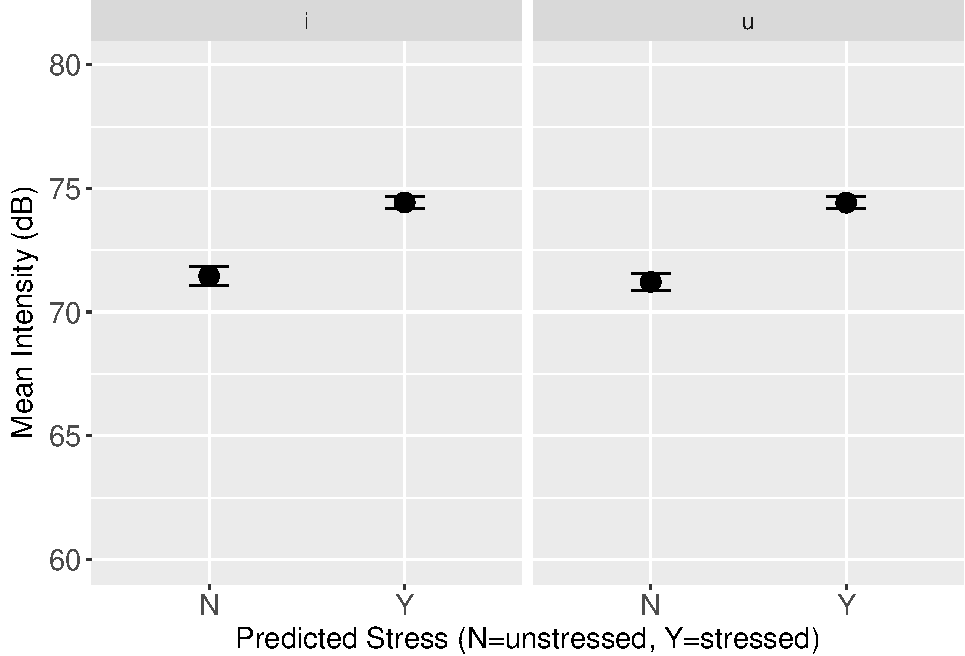
\includegraphics{lithuanian_article_files/figure-latex/Figure3-1.pdf}
\caption{\label{fig:Figure3}Mean Intensity in dB by Predicted Stress
(N=unstressed, Y=stressed), {[}u{]} and {[}i{]}}
\end{figure}

Across frame sentence and syllable count, stressed and unstressed
{[}u{]} displayed a mean intensity difference of approximately 3 dB
(74.5 dB (2.44 dB s.d.) and 71.4 dB (3.13 dB s.d.), respectively). These
mean estimates remained stable for intensity measurements on {[}u{]}
vowels in both frame sentences and within three- and four-syllable
words, as shown in \textit{Table 3}. Model comparison yielded an effect
of predicted stress on the intensity parameter for the {[}u{]} vowel
(\(\chi^2(1) = 58.289, p < 0.05\)), such that stress on {[}u{]}
indicates an estimated intensity increase of 3.27 dB +/- 0.37 dB
(standard error).

\begin{table}

\caption{\label{tab:Table3}Intensity in dB by Predicted Stress (Stress), Frame Sentence (Frame), and Syllable Count (Syllnum), [u] Vowel}
\centering
\begin{tabular}[t]{l|r|l|r|r}
\hline
Stress & Frame & Syllnum & Mean & SD\\
\hline
N & 1 & four & 72.78 & 3.51\\
\hline
N & 1 & three & 71.59 & 2.82\\
\hline
N & 2 & four & 71.77 & 3.28\\
\hline
N & 2 & three & 70.59 & 3.17\\
\hline
Y & 1 & four & 75.35 & 1.94\\
\hline
Y & 1 & three & 74.31 & 2.63\\
\hline
Y & 2 & four & 74.62 & 2.89\\
\hline
Y & 2 & three & 74.49 & 2.24\\
\hline
\end{tabular}
\end{table}

Similar results were observed for {[}i{]}. Intensity values for this
vowel closely mirror the {[}u{]} vowel data, with a corresponding 3 dB
gap between mean intensity values on stressed (74.5 dB (2.55 dB s.d.))
and unstressed (17.5 dB (2.79 dB s.d.)) syllables. Comparison of the
intensity models fit to the {[}i{]} vowel data yielded a main effect of
predicted stress (\(\chi^2(1) = 39.409, p < 0.05\)). Again, these
results were almost identical to the {[}u{]} vowel data; word stress
correlates with an estimated 3.28 dB (+/- 0.47 dB standard error)
increase in intensity on {[}i{]} vowels.

\begin{table}

\caption{\label{tab:Table4}Intensity in dB by Predicted Stress (Stress), Frame Sentence (Frame), and Syllable Count (Syllnum), [i] Vowel}
\centering
\begin{tabular}[t]{l|r|l|r|r}
\hline
Stress & Frame & Syllnum & Mean & SD\\
\hline
N & 1 & four & 71.60 & 2.57\\
\hline
N & 1 & three & 72.50 & 2.72\\
\hline
N & 2 & four & 70.33 & 2.50\\
\hline
N & 2 & three & 70.95 & 3.01\\
\hline
Y & 1 & four & 73.89 & 2.61\\
\hline
Y & 1 & three & 74.72 & 2.67\\
\hline
Y & 2 & four & 74.30 & 2.79\\
\hline
Y & 2 & three & 75.04 & 2.14\\
\hline
\end{tabular}
\end{table}

\subsection{F1 and F2}\label{f1-and-f2}

In general, reliability of vowel quality (measured in F1 and F2) as an
acoustic correlate of stress would predict discrepancies between F1 and
F2 depending on the vowel. In the case of the high, back vowel {[}u{]},
centralization of an unstressed vowel corresponds to relatively higher
F1 and higher F2. Centralization of the high, front vowel {[}i{]}, by
contrast, is realized with higher F1 and lower F2. Peripheralization of
a stressed vowel would predict the inverse (lower F1/lower F2 for
{[}u{]}; lower F1/higher F2 for {[}i{]}).

Turning to the extracted vowel quality data, little variation was
observed for {[}u{]} in stressed and unstressed syllables for either
mean F1 or mean F2. F1 values were almost identical (416 Hz (68.7 Hz
s.d.) in unstressed syllables; 413 Hz (67.3 Hz s.d.) in stressed
syllables), while F2 values were higher for unstressed syllables (1247
Hz (362 Hz s.d.)) than stressed syllables (1091 Hz (342 Hz s.d.)).
Grouping by frame sentence and by-word syllable count
(\textit{Table 5}), however, reveals substantial overlap between F1 and
F2 figures in stressed and unstressed environments. A vowel plot for
stressed and unstressed {[}u{]} in trisyllabic words in
\textit{Figure 4} illustrates this overlap; in the figure, vowels marked
\enquote{u2} and \enquote{u5} represent {[}u{]} vowels in unstressed
syllables in the first and second frame sentence, respectively, while
\enquote{U2} and \enquote{U5} indicate vowels in stressed syllables in
the first and second frame sentence, respectively.

\begin{table}

\caption{\label{tab:Table5}F1 and F2 in Hz by Predicted Stress (Stress), Frame Sentence (Frame), and Syllable Count (Syllnum), [u] Vowel}
\centering
\begin{tabular}[t]{l|r|l|r|r|r|r}
\hline
Stress & Frame & Syllnum & F1 Mean & F1 SD & F2 Mean & F2 SD\\
\hline
N & 1 & four & 391.92 & 56.22 & 1061.12 & 273.52\\
\hline
N & 1 & three & 412.99 & 74.74 & 1209.89 & 340.21\\
\hline
N & 2 & four & 448.34 & 97.11 & 1308.99 & 473.69\\
\hline
N & 2 & three & 415.44 & 53.30 & 1322.63 & 357.97\\
\hline
Y & 1 & four & 429.93 & 99.92 & 1106.91 & 546.28\\
\hline
Y & 1 & three & 418.43 & 68.92 & 1160.00 & 376.57\\
\hline
Y & 2 & four & 400.82 & 33.63 & 961.73 & 164.24\\
\hline
Y & 2 & three & 407.43 & 62.91 & 1062.02 & 253.99\\
\hline
\end{tabular}
\end{table}

\begin{figure}
\centering
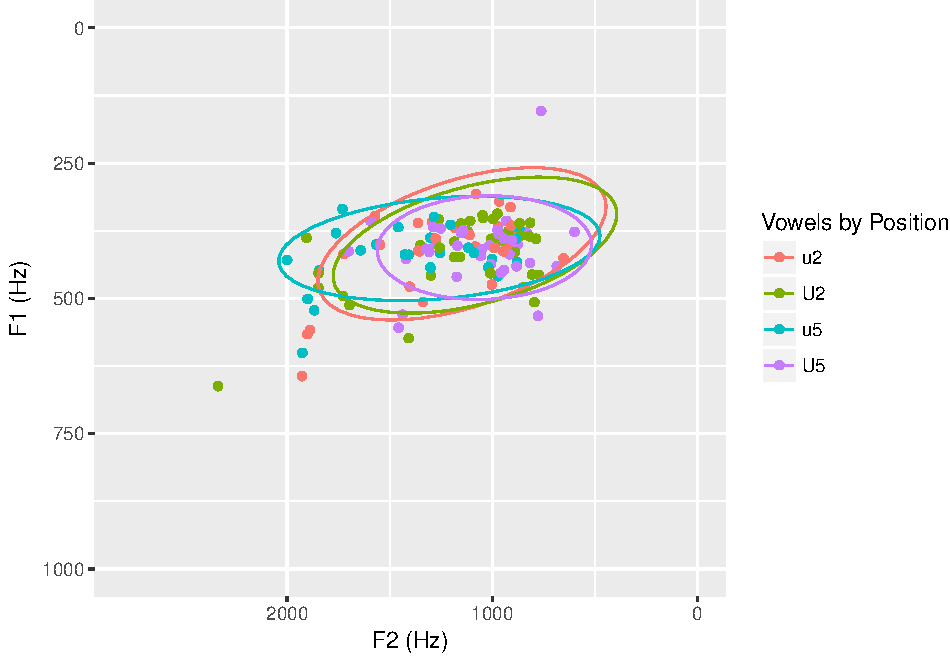
\includegraphics{lithuanian_article_files/figure-latex/Figure4-1.pdf}
\caption{\label{fig:Figure4}F1/F2 Plot, {[}u{]} Vowel (Trisyllabic Words)}
\end{figure}

Separate sets of linear mixed effects models were fit to the F1 and F2
data for {[}u{]}. Nested model comparison did not identify predicted
stress as a main effect for either F1 (\(\chi^2(1) = 1.59, p = 0.2062\))
or F2 (\(\chi^2(1) = 2.7143, p = 0.0995\)).

Mean F1 and F2 values remained mostly uniform across stressed and
unstressed syllables containing a {[}i{]} nucleus. Less than a 10 Hz
mean change was observed for F1 (unstressed: 369 Hz (35.5 Hz s.d.);
stressed: 376 Hz (32.3 Hz s.d.)), and mean F2 values varied by less than
100 Hz (unstressed: 1621 Hz (228 Hz s.d.); stressed: 1696 Hz (183 Hz
s.d.)). The range of values for both parameters are spread evenly across
{[}i{]} vowels in each frame sentence and for three- and four-syllable
words (see \textit{Table 6}). \textit{Figure 5} demonstrates the
homogeneity of the vowel quality data with a vowel plot of trisyllabic
words containing a {[}i{]} nucleus; substantial intersection in the
vowel space of stressed and unstressed syllables is evident (the same
labeling schema from \textit{Figure 4} holds).

\begin{table}

\caption{\label{tab:Table6}F1 and F2 in Hz by Predicted Stress (Stress), Frame Sentence (Frame), and Syllable Count (Syllnum), [i] Vowel}
\centering
\begin{tabular}[t]{l|r|l|r|r|r|r}
\hline
Stress & Frame & Syllnum & F1 Mean & F1 SD & F2 Mean & F2 SD\\
\hline
N & 1 & four & 390.04 & 37.98 & 1536.73 & 256.18\\
\hline
N & 1 & three & 355.31 & 27.85 & 1712.59 & 191.61\\
\hline
N & 2 & four & 382.69 & 38.29 & 1475.63 & 234.46\\
\hline
N & 2 & three & 360.21 & 32.17 & 1672.65 & 190.02\\
\hline
Y & 1 & four & 386.69 & 34.22 & 1674.45 & 176.81\\
\hline
Y & 1 & three & 360.50 & 32.08 & 1789.56 & 143.83\\
\hline
Y & 2 & four & 388.68 & 30.67 & 1588.71 & 195.52\\
\hline
Y & 2 & three & 370.20 & 25.00 & 1714.34 & 169.62\\
\hline
\end{tabular}
\end{table}

\begin{figure}
\centering
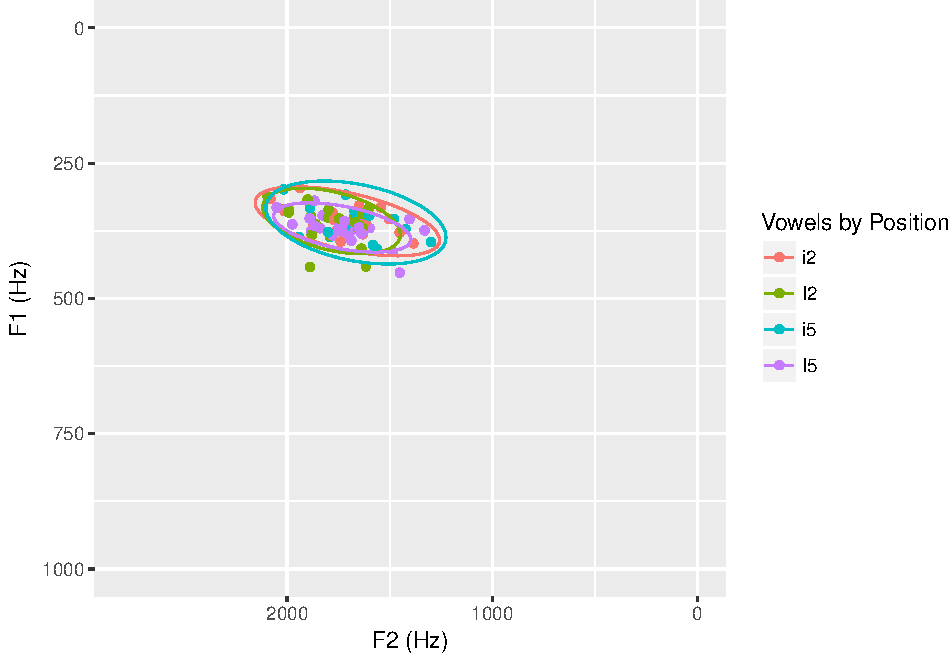
\includegraphics{lithuanian_article_files/figure-latex/Figure5-1.pdf}
\caption{\label{fig:Figure5}F1/F2 Plot, {[}i{]} Vowel (Trisyllabic Words)}
\end{figure}

Surprisingly, nested model comparison of the F1 models on {[}i{]}
revealed that vowel quality does vary as a function of predicted stress
(\(\chi^2(1) = 4.127, p = 0.0422\)), such that F1 on {[}i{]} vowels in
stressed syllables increases by an estimated 11.19 Hz +/- 5.2 Hz
(standard error). The same effect was not observed for F2
(\(\chi^2(1) = 0.7222, p = 0.3954\)).

\subsection{F0}\label{f0}

\textit{Figure 6} plots mean F0 values for {[}u{]} and {[}i{]} vowels
across stressed and unstressed syllables. The general trend is toward
higher F0 on stressed syllables, and lower F0 on unstressed syllables.

\begin{figure}
\centering
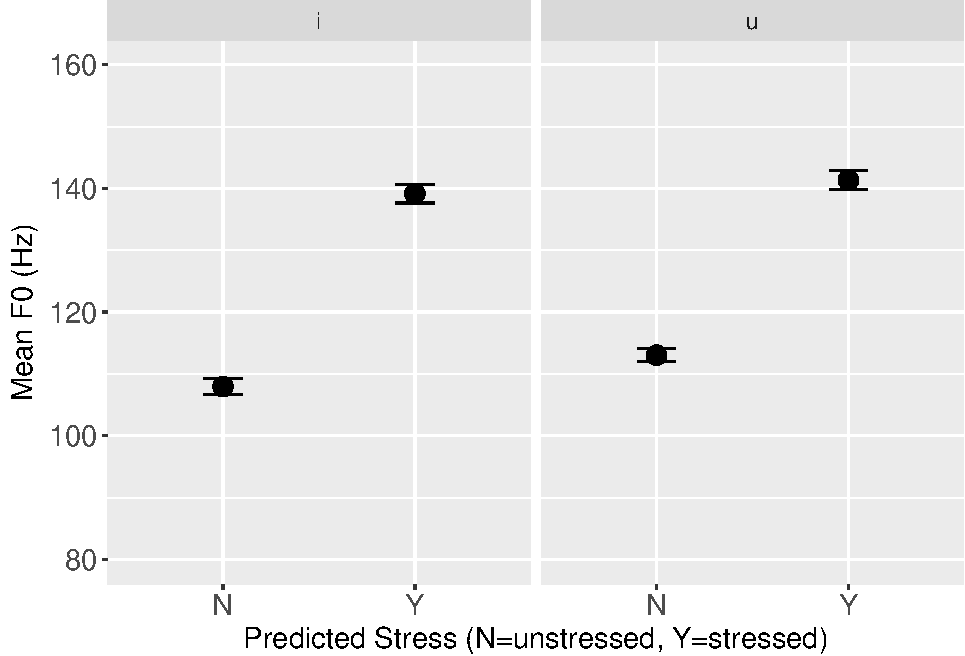
\includegraphics{lithuanian_article_files/figure-latex/Figure6-1.pdf}
\caption{\label{fig:Figure6}Mean F0 in Hz by Predicted Stress (N=unstressed,
Y=stressed), {[}u{]} and {[}i{]}}
\end{figure}

Examining mean figures for all {[}u{]} vowels, variation in F0 as a
function of stress was approximately 46 Hz (unstressed: 113 Hz (9.49 Hz
s.d.); stressed: 159 Hz (25.1 Hz s.d.)). This tendency is mostly uniform
across {[}u{]} vowels in both frame sentences and within three- and
four-syllable words (see \textit{Table 7}). Comparison of the linear
mixed effects models fit to the data indicated a main effect of
predicted stress (\(\chi^2(1) = 121.1, p < 0.05\)); stress on the vowel
raises F0 by an estimated 43.029 Hz +/- 2.71 Hz (standard error).

\begin{table}

\caption{\label{tab:Table7}F0 in Hz by Predicted Stress (Stress), Frame Sentence (Frame), and Syllable Count (Syllnum), [u] Vowel}
\centering
\begin{tabular}[t]{l|r|l|r|r}
\hline
Stress & Frame & Syllnum & Mean & SD\\
\hline
N & 1 & four & 120.73 & 8.14\\
\hline
N & 1 & three & 117.94 & 8.41\\
\hline
N & 2 & four & 105.81 & 8.15\\
\hline
N & 2 & three & 108.11 & 6.77\\
\hline
Y & 1 & four & 148.59 & 19.88\\
\hline
Y & 1 & three & 150.10 & 20.31\\
\hline
Y & 2 & four & 168.81 & 26.73\\
\hline
Y & 2 & three & 168.51 & 26.41\\
\hline
\end{tabular}
\end{table}

Similar effects were observed for {[}i{]} vowels, whose mean F0 values
varied approximately 39 Hz across stressed and unstressed syllables
(unstressed: 108 Hz (9.46 Hz s.d.); stressed: 147 Hz (20 Hz s.d.)).
\textit{Table 8} illustrates that this variation is sustained in both
frame sentences and across words of varying lengths. Additionally, model
comparison identified predicted stress as a main effect
(\(\chi^2(1) = 88.482, p < 0.05\)) such that {[}i{]} vowels on stressed
syllables correlate with an increase in F0 of approximately 36.349 Hz
+/- 2.733 Hz (standard error).

\begin{table}

\caption{\label{tab:Table8}F0 in Hz by Predicted Stress (Stress), Frame Sentence (Frame), and Syllable Count (Syllnum), [i] Vowel}
\centering
\begin{tabular}[t]{l|r|l|r|r}
\hline
Stress & Frame & Syllnum & Mean & SD\\
\hline
N & 1 & four & 112.12 & 10.11\\
\hline
N & 1 & three & 113.12 & 7.37\\
\hline
N & 2 & four & 104.15 & 11.06\\
\hline
N & 2 & three & 101.99 & 5.11\\
\hline
Y & 1 & four & 143.34 & 19.64\\
\hline
Y & 1 & three & 140.25 & 10.42\\
\hline
Y & 2 & four & 153.27 & 23.28\\
\hline
Y & 2 & three & 152.17 & 22.49\\
\hline
\end{tabular}
\end{table}

\section{Discussion}\label{discussion}

The current study examined five acoustic measures which have been
claimed to signal word stress in Lithuanian: normalized duration,
intensity, F1, F2, and F0.

Analysis of the normalized duration results confirms Hypothesis 1.
{[}u{]} and {[}i{]} vowels on syllables predicted to be stressed were
longer than those in unstressed syllables by an estimated 11.62 ms and
12.85 ms, respectively. Not only was this difference found to be
significant, but it is also likely to be perceptible to hearers.
Assuming even a conservative Just-Noticeable-Difference for duration of
20\% (Klatt (1976)), the parameter estimates yielded by duration models
for both vowels surpass this perceptibility threshold. Therefore,
duration is a reliable acoustic correlate of stress on {[}u{]} and
{[}i{]} vowels for this speaker.

Intensity results, similarly, confirm Hypothesis 2. For both vowels,
greater intensity was observed in stressed syllables than in unstressed
syllables. Model comparison revealed a main effect of predicted stress
such that vowels on stressed syllables are produced with an intensity
level 3 dB greater than unstressed syllables. Again, this difference is
perceptible to hearers (Harris (1963)), indicating that intensity
reliably marks stress on {[}u{]} and {[}i{]} in the speech of the
experiment participant.

The vowel quality data as a whole fail to confirm Hypothesis 3. Stressed
vowels did not show evidence of peripheralization compared to vowels in
unstressed syllables. A main effect of stress on the realization of F1
was found for the vowel {[}i{]}; however, this increase in F1 as a
function of stress represents a lowering of {[}i{]} in the vowel space,
which is the \emph{opposite} of what the hypothesis would predict for
that vowel. Furthermore, the 11 Hz parameter estimate for the model is
negligible. Given these facts, vowel quality (measured by F1 and F2) is
demonstrably unreliable as an acoustic correlate of word stress for the
experiment participant. This result contradicts previous accounts of the
phonetic realization of stress in Lithuanian.

F0 data indicate that stress correlates with higher pitch for both
{[}u{]} and {[}i{]}. Model comparison revealed a main effect of
predicted stress on the realization of F0, and the predicted increases
were comparable for each vowel. This suggests evidence in support of
Hypothesis 4.

\begin{figure}
\centering
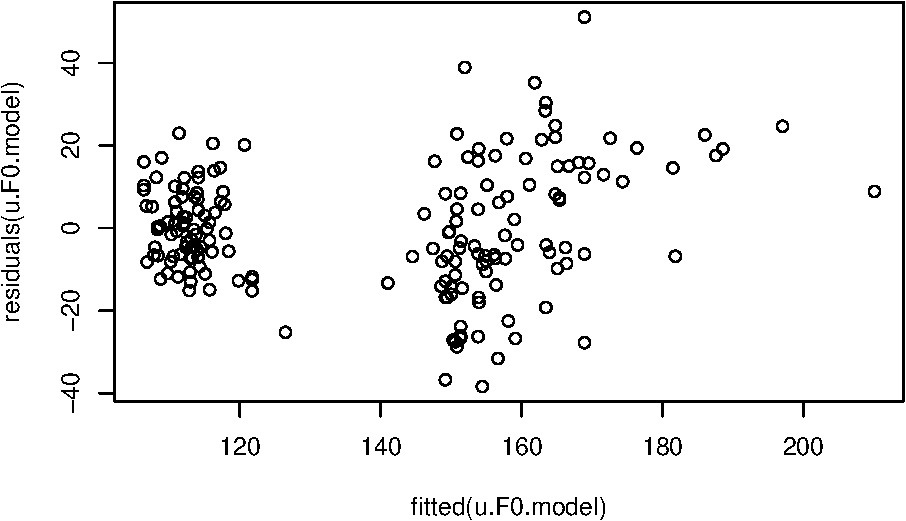
\includegraphics{lithuanian_article_files/figure-latex/Figure7-1.pdf}
\caption{\label{fig:Figure7}Heteroskedastic residuals for F0 LME model,
{[}u{]} vowel}
\end{figure}

In evaluating the reliability of these models, however, it was
discovered that residuals for both {[}u{]} and {[}i{]} F0 models
violated homoskedasticity, as shown in \textit{Figure7} and
\textit{Figure 8}. Two distinct distributional regions are clear from
these residual plots. New models were fit to the data using a
log-transformed F0 predictor in an attempt to mitigate this effect.
Nested model comparisons for these models revealed a main effect of
predicted stress, much like for the unstransformed F0 models. Again,
however, visual inspection of residuals determined a violation of the
homoskedasticity assumption.

\begin{figure}
\centering
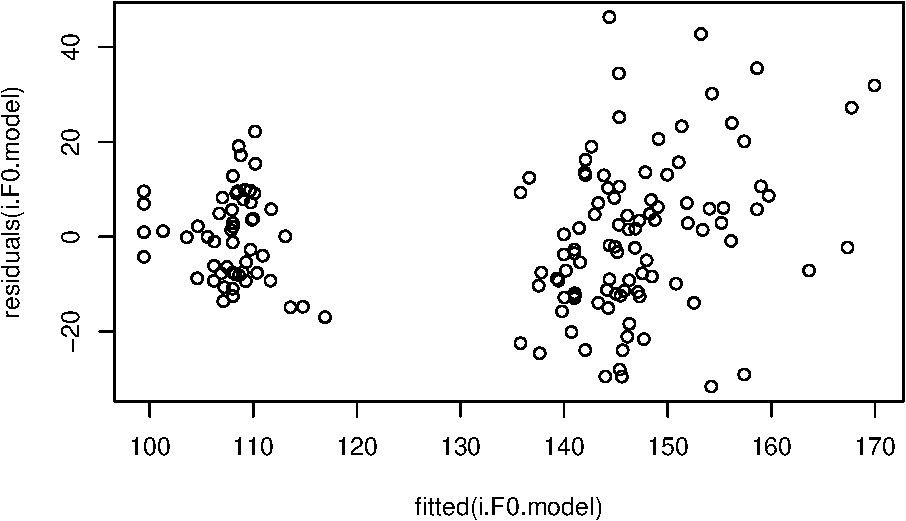
\includegraphics{lithuanian_article_files/figure-latex/Figure8-1.pdf}
\caption{\label{fig:Figure8}Heteroskedastic residuals for F0 LME model,
{[}i{]} vowel}
\end{figure}

At least two explanations are possible for this result. One is that
there exists another variable (or variables) unaccounted for in the
models beyond frame sentence, segmental environment, number of
syllables, and repetition. Another possibility assumes Generative
analyses of grave syllables--that is, that they bear tone--and that F0
is realizing a categorical tonal distinction (between a {[}H{]} target
and a {[}L{]} target or default toneless target; recall that tonal
distinctions are neutralized in unstressed position). Under this
assumption, the expectation of a bimodal distribution of the F0 data is
reasonable, with local maxima corresponding to {[}H{]} and {[}L{]} (or
default toneless) targets. Histograms of the F0 data for both {[}u{]}
and {[}i{]} (\textit{Figure 9} and \textit{Figure 10}) are inconclusive,
however; F0 values in stressed and unstressed syllables appear to
congregate around local maxima, but with a substantial degree of
overlap, particularly for {[}i{]}. Data from additional native speakers
will be necessary to determine the nature and robustness of this effect.

\begin{figure}
\centering
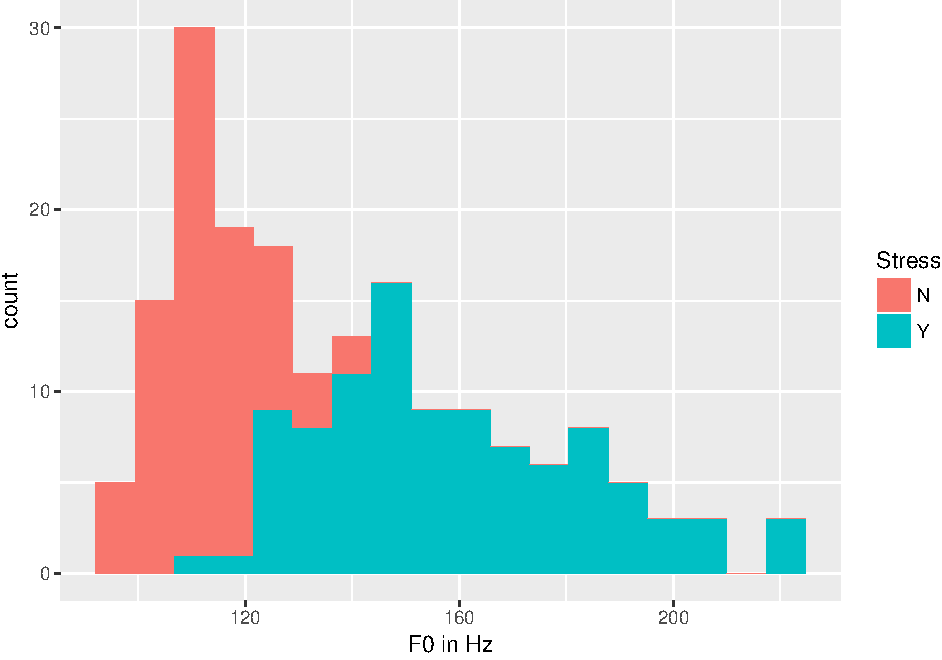
\includegraphics{lithuanian_article_files/figure-latex/Figure9-1.pdf}
\caption{\label{fig:Figure9}Histogram of F0 Values Separated by Stress,
{[}u{]} Vowel}
\end{figure}

\begin{figure}
\centering
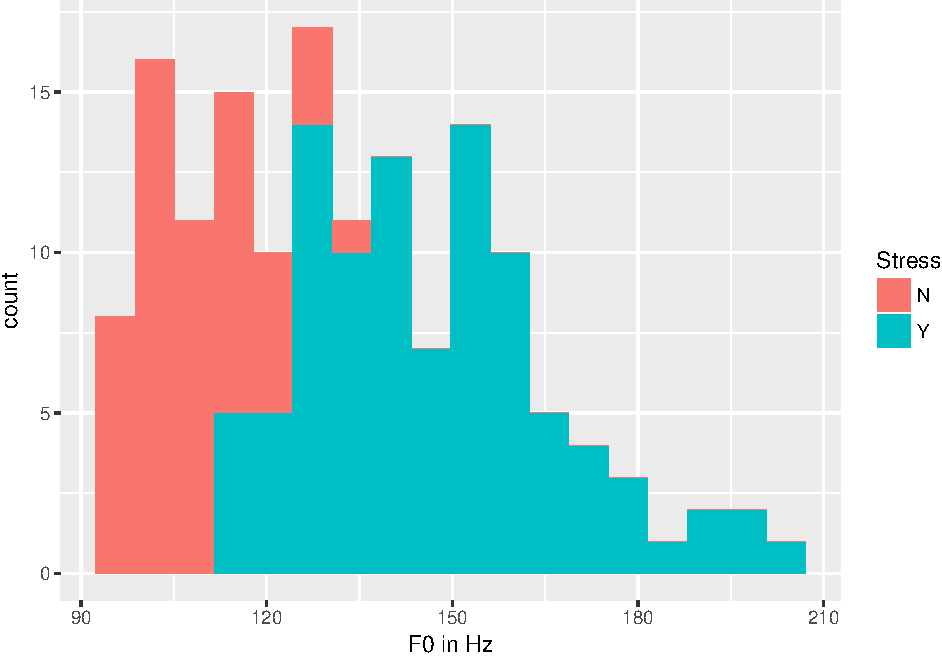
\includegraphics{lithuanian_article_files/figure-latex/Figure10-1.pdf}
\caption{\label{fig:Figure10}Histogram of F0 Values Separated by Stress,
{[}i{]} Vowel}
\end{figure}

To assess the cumulative reliability of the separate linear mixed
effects models for acoustic parameter, a logistic regression model was
fit to each vowel (using the \emph{glmer()} function in lme4). Predicted
stress (categorical variable with two levels: stressed and unstressed)
was set as the criterion, with the five acoustic correlates as
continuous predictors (normalized duration, intensity, F1, F2, F0).
Acoustic data were rescaled using the \emph{scale()} function. Models
for both vowels failed to converge with a fully-specified random effects
structure, that is, by-word random slopes for frame sentence, segmental
environment, number of syllables in the word, as well as repetition. A
majority of the possible minimally-specified permutations of these
effects also failed to reach convergence. For {[}u{]}, two models
converged: one specifying by-word random slopes for repetition, and one
for frame sentence. Three models converged for {[}i{]}: one specifying
by-word random slopes for repetition, one for frame, and one which
included both. For all five models, intercepts were uncorrelated in the
random effects structure.

The logistic regression models on {[}u{]} indicate a main effect of F0
(repetition model:
\(\beta = 7.028, \, se = 2.056, \ z=3.149, \, p<0.05\); frame sentence
model: \(\beta = 7.5989, \, se = 2.3196, \ z=3.276, \, p<0.05\)), but
only a marginally-significant effect of normalized duration (repetition
model: \(\beta = 0.9959, \, se = 0.5251, \ z=1.897, \, p = 0.058\);
frame sentence model:
\(\beta = 0.991, \, se = .5283, \ z=1.875, \, p=0.061\)). No main
effects were observed for intensity, F1, or F2.

The three models fit to {[}i{]} data revealed main effects of both F0
and normalized duration (see \textit{Table 9}). No effects were observed
for intensity, F1, or F2.

\begin{table}
\begin{center}
\caption{Logistic Regression Models, [i]}
\begin{tabular}{r|cccc}
& $\beta$ & $se$ & $z$ & $p$ \\
\hline \
\textbf{Repetition Model} \\
F0 & 7.44 & 2.02 & 3.68 & <0.05 \\
Duration & 1.44 & 0.56 & 2.56 & <0.05 \\
\hline
\textbf{Frame Sentence Model} \\
F0 & 8.13 & 3.25 & 2.5 & <0.05 \\
Duration & 1.51 & 0.67 & 2.26 & <0.05 \\
\hline
\textbf{Repetition+Frame Model} \\
F0 & 8.05 & 2.36 & 3.42 & <0.05 \\
Duration & 1.58 & 0.66 & 2.4 & <0.05 \\
\end{tabular}
\end{center}
\end{table}

These results are mostly consistent with the linear mixed effects models
in that duration and pitch are reliable predictors of predicted stressed
position, while vowel quality is not. The one exception is intensity.
This discrepancy may be due to the effect of variable rescaling; the 3
dB difference estimated by the linear effects models (determined to be
significant and perceptible to hearers) may have been minimized during
rescaling to allow for comparison with other values measured in
milliseconds and Hertz. Another unfortunate tradeoff for model
convergence was the thinning of the random effects structure,
potentially impacting the accuracy of the logistic regression models. A
larger data set (with multiple speakers) may rectify this issue,
allowing for more complete random effects specification.

\section{Conclusion}\label{conclusion}

This study has addressed the question \enquote{What is stress in a tone
language?} by examining the acoustic correlates of stress on grave
syllables in Lithuanian nominals. The results of a production study
partially confirmed previous accounts of stress in the language:
stressed syllables are marked by longer duration and greater intensity
on vowels, but not by changes in vowel quality. Vowels on stressed
syllables were realized with higher F0, but it is unclear whether this
is an acoustic correlate of stress or a lexical tonal contrast. A larger
dataset will provide a frame of reference in confirming the effects
observed in this study.

\newpage

\section{References}\label{references}

\setlength{\parindent}{-0.5in} \setlength{\leftskip}{0.5in}

\hypertarget{refs}{}
\hypertarget{ref-Ambrazas97}{}
Ambrazas, V. (Ed.). (1997). \emph{Lithuanian grammar}. Vilnius,
Lithuania: Baltos Lankos.

\hypertarget{ref-R-lme4}{}
Bates, D., Mächler, M., Bolker, B., \& Walker, S. (2015). Fitting linear
mixed-effects models using lme4. \emph{Journal of Statistical Software},
\emph{67}(1), 1--48.
doi:\href{https://doi.org/10.18637/jss.v067.i01}{10.18637/jss.v067.i01}

\hypertarget{ref-Blevins93}{}
Blevins, J. (1993). A tonal analysis of lithuanian nominal accent.
\emph{Language}, \emph{69}, 237--273.

\hypertarget{ref-Praat}{}
Boersma, P., \& Weenink, D. (2016). \emph{Praat: Doing phonetics by
computer}. Retrieved from \url{https://praat.org/}

\hypertarget{ref-deLacy02}{}
deLacy, P. (2002). The interaction of tone and stress in optimality
theory. \emph{Phonology}, \emph{19}, 1--32.

\hypertarget{ref-Dogil99}{}
Dogil, G. (1999). Baltic languages. In H. van der Hulst (Ed.),
\emph{Word prosodic systems in the languages of europe} (pp. 877--897).
Berlin: Mouton de Gruyter.

\hypertarget{ref-Francisetal02}{}
Francis, A., Ciocca, V., \& Yu, J. M. C. (2002). Accuracy and
variability of acoustic measures of voicing onset. \emph{Journal of the
Acoustical Society of America}, \emph{113}, 1025--1032.

\hypertarget{ref-Girdenis03}{}
Girdenis, A. (Ed.). (2003). \emph{Teorinai lietuviu fonologijos
pagrindai {[}theoretical foundations of lithuanian phonology{]}}.
Vilnius, Lithuania: Mokslo Ir Enciklopediju Leidybos Institutas.

\hypertarget{ref-Gordon_Roettger17}{}
Gordon, M., \& Roettger, T. (2017). Loudness acoustic correlates of word
stress: A cross-linguistic survey. \emph{Linguistics Vanguard},
\emph{3}.

\hypertarget{ref-Harris63}{}
Harris, D. J. (1963). Loudness discrimination. \emph{Journal of Speech
and Hearing Disorders}.

\hypertarget{ref-Kenstowicz72}{}
Kenstowicz, M. (1972). Lithuanian phonology. \emph{Studies in the
Linguistic Sciences}, \emph{2}, 1--85.

\hypertarget{ref-Klatt76}{}
Klatt, D. H. (1976). Linguistic uses of segmental duration in english:
Acoustic and perceptual evidence. \emph{Journal of the Acoustical
Society of America}, \emph{59}, 1208--1221.

\hypertarget{ref-Lennes03}{}
Lennes, M. (2003). \emph{Collect\_formant\_data\_from\_files.praat}.
Retrieved from \url{https://www.helsinki.fi/~lennes/praat/scripts/}

\hypertarget{ref-Mathiassen96}{}
Mathiassen, T. (1996). \emph{A short grammar of lithuanian}. Columbus,
OH: Slavica Publishers.

\hypertarget{ref-R-base}{}
R Core Team. (2017). \emph{R: A language and environment for statistical
computing}. Vienna, Austria: R Foundation for Statistical Computing.
Retrieved from \url{https://www.R-project.org/}

\hypertarget{ref-Turketal06}{}
Turk, A., Nakai, S., \& Sugahara, M. (2006). Acoustic segment durations
in prosodic research: A practical guide. In S. Sudhoff, D. Lenertova, R.
Meyer, S. Pappert, P. Augurzky, I. Mleinek, \ldots{} J. Schlieser
(Eds.), \emph{Methods in empirical prosody research} (pp. 1--28).
Berlin: Mouton de Gruyter.

\hypertarget{ref-Wightmanetal92}{}
Wightman, C. W., Shattuck-Hufnagel, S., Ostendorf, M., \& Price, P. J.
(1992). Segmental durations in the vicinity of prosodic phrase
boundaries. \emph{Journal of the Acoustical Society of America},
\emph{92}, 1707--1717.

\hypertarget{ref-Young91}{}
Young, S. R. (1991). \emph{The prosodic structure of lithuanian}.
University Press of America.






\end{document}
